%%%%%%%%%%%%%%%%%%%%%%%%%%%%%%%%%%%%%%%%%%%%%%%%%%%%%%%%%%%%%%%%%%%%%%%%%%%
% Chapter: Sample and Hold
% Falstad examples: examples/samplehold (generated by falstad/circuits/samplehold.py)
% Common values (capstone): fs = 5 Hz, clock duty 10 % (track 20 ms, hold
% 180 ms), RS = 1 kOhm, Ron = 20 Ohm, CH = 1 uF, 3 bit, 0..4 V, LSB 0.5 V
%%%%%%%%%%%%%%%%%%%%%%%%%%%%%%%%%%%%%%%%%%%%%%%%%%%%%%%%%%%%%%%%%%%%%%%%%%%

%%%%%%%%%%%%%%%%%%%%%%%%%%%%%%%%%%%%%%%%%%%%%%%%%%%%%%%%%%%%%%%%%%%%%%%%%%%
\section{Why Sample and Hold?}
%%%%%%%%%%%%%%%%%%%%%%%%%%%%%%%%%%%%%%%%%%%%%%%%%%%%%%%%%%%%%%%%%%%%%%%%%%%
\nsl{The previous chapters produced a clean, filtered analog voltage. The
next step is to turn it into numbers. A digital system cannot store a
continuous signal; it takes one value per sampling period and works with
this sequence of numbers. The circuit that takes these values is the
\emph{sample and hold} (S\&H) stage. It sits between the anti-aliasing
filter and the analog-to-digital converter (ADC).
\newline
The S\&H stage has two jobs. First, it defines the \emph{sampling
instant}: the moment at which the signal is measured. Second, it keeps the
measured voltage constant while the converter works on it. Many converters
need some time for a conversion and give wrong results if their input
changes during this time. A successive-approximation converter, for
example, compares the input with a sequence of trial voltages; if the input
moves in between, the result is a mixture of different input values.
\newline
In the lab and in the capstone task the sampling frequency is very low,
$f_s=\SI{5}{\hertz}$, so that we can follow every sample by eye on the
Falstad scope and on the LEDs. The principles are the same as in a
converter with millions of samples per second, only the time scales
differ \cite{kester2005,razavi1995}.\newpage}

\begin{description}
\item[{\rot\bf Position in the signal chain}]~\\[-\lblskip]
\begin{center}
\resizebox{0.9\textwidth}{!}{%
\begin{tikzpicture}[font=\sffamily\small,>=Stealth,
	b/.style={draw,thick,minimum height=11mm,minimum width=22mm,align=center}]
	\node[b,fill=gray!10] (s1) at (0,0) {sensor \&\\conditioning};
	\node[b,fill=rwucyan!10] (s2) at (3.4,0) {anti-aliasing\\low-pass};
	\node[b,fill=rwuviolet!15] (s3) at (6.8,0) {\textbf{sample}\\\textbf{\& hold}};
	\node[b,fill=rwucyan!10] (s4) at (10.2,0) {ADC};
	\node[b,fill=gray!10] (s5) at (13.6,0) {digital\\value};
	\draw[->,thick] (s1) -- (s2);
	\draw[->,thick] (s2) -- (s3);
	\draw[->,thick] (s3) -- (s4);
	\draw[->,thick] (s4) -- node[above]{\scriptsize $N$ bit} (s5);
	\draw[->,thick] (6.8,-1.6) node[below]{clock $f_s$} -- (s3);
	\draw[->,thick] (10.2,-1.6) node[below]{start / clock} -- (s4);
\end{tikzpicture}}
\end{center}
\bi
	\ite the S\&H stage \textbf{defines the sampling instant} $t_k = k\,T_s$, $T_s = 1/f_s$
	\ite it keeps the voltage \textbf{constant while the ADC converts}
	\ite capstone: $f_s = \SI{5}{\hertz}$, 3-bit flash converter, full scale \SI{4}{\volt}
\ei
\os{\newpage}

\item[{\rot\bf What goes wrong without S\&H}]~\\[-\lblskip]
\bi
	\ite the input changes during the conversion time $t_\mathrm{conv}$
	\ite the error must stay below $\frac12\,\LSB$:
	$\displaystyle \left|\frac{dV}{dt}\right|_\mathrm{max}\, t_\mathrm{conv} < \frac12\,\LSB$
	\ite sine $V(t) = \hat V \sin(2\pi f t)$: maximum slope $2\pi f \hat V$
	\ite example: 12-bit ADC, \SI{4}{\volt} full scale ($\LSB = \SI{0.98}{\milli\volt}$), $t_\mathrm{conv} = \SI{10}{\micro\second}$, $\hat V=\SI{2}{\volt}$
	\bi
		\itee $f < \frac{\LSB/2}{2\pi \hat V t_\mathrm{conv}} = \SI{3.9}{\hertz}$ without S\&H
		\itee with S\&H only the much shorter \emph{aperture time} counts (nanoseconds)
	\ei
	\ite a \textbf{flash} converter decides in one step, but the digital outputs still have to be read and displayed at a defined instant
\ei
\nsl{The example shows how strict the requirement is. A 12-bit converter
without S\&H can only follow signals of a few hertz, even though its
conversion time is short. With an S\&H stage in front, the relevant time is
the uncertainty of the sampling instant, which is many orders of magnitude
shorter. In our capstone the flash converter is fast, but the S\&H stage
still gives us one well-defined value per \SI{200}{\milli\second}, so that
the display does not flicker and the digital code belongs to a known
instant.}
\os{\newpage}
\end{description}

%%%%%%%%%%%%%%%%%%%%%%%%%%%%%%%%%%%%%%%%%%%%%%%%%%%%%%%%%%%%%%%%%%%%%%%%%%%
\section{The Track-and-Hold Principle}
%%%%%%%%%%%%%%%%%%%%%%%%%%%%%%%%%%%%%%%%%%%%%%%%%%%%%%%%%%%%%%%%%%%%%%%%%%%
\nsl{The simplest S\&H stage is a switch and a capacitor. While the switch
is closed, the capacitor voltage follows the input (track mode). When the
switch opens, the capacitor keeps its charge and therefore its voltage
(hold mode). Strictly speaking this circuit is a \emph{track-and-hold}
circuit, because it follows the input during the whole time the switch is
closed. A true sample-and-hold would take a very short sample. In practice
the two names are used for the same circuit.\newpage}

\begin{description}
\item[{\rot\bf Switch and hold capacitor}]~\\[-\lblskip]
\begin{center}
\begin{circuitikz}[scale=0.9, transform shape]
  \draw (0,0) node[ground]{} to[sV, l=$\Vin$] (0,2.5)
        to[R, l=$R_S$] (2.5,2.5)
        to[nos, l=$S$, name=sw] (4.5,2.5) -- (5.5,2.5)
        to[C, l=$C_H$] (5.5,0) node[ground]{};
  \draw (5.5,2.5) to[short,*-o] (7,2.5) node[right]{$V_H$};
  \draw (sw.north) ++(0,0.3) -- ++(0,0.8) node[above]{clock};
\end{circuitikz}
\end{center}
\bi
	\ite clock high: switch closed, $C_H$ follows $\Vin$ (\textbf{track})
	\ite clock low: switch open, $C_H$ keeps its charge (\textbf{hold})
	\ite capstone clock: \SI{5}{\hertz}, duty cycle \SI{10}{\percent}: track \SI{20}{\milli\second}, hold \SI{180}{\milli\second}
\ei
\nsl{$R_S$ is the total resistance in the charging path. It contains the
output resistance of the source, the on-resistance of the switch and, in
our circuits, a resistor of \SI{1}{\kilo\ohm} that limits the charging
current of the op-amp that drives the capacitor.}
\os{\newpage}

\item[{\rot\bf Timing diagram}]~\\[-\lblskip]
\begin{center}
\begin{tikzpicture}
\begin{axis}[width=12cm,height=4.6cm,xmin=0,xmax=2,ymin=0,ymax=4.2,
	xlabel={$t$ / s},ylabel={$V$ / V},axis lines=left,font=\scriptsize,
	xtick={0,0.2,...,2.0},xticklabel style={/pgf/number format/fixed},
	legend style={at={(1,1)},anchor=north east,draw=none,fill=none},
	legend columns=2]
\addplot[rwucyan,thick,domain=0:2,samples=101] {2+1.5*sin(deg(pi*x))};
\addlegendentry{$\Vin$}
\addplot[rwuviolet,very thick,const plot,domain=0:2,samples=11] {2+1.5*sin(deg(pi*x))};
\addlegendentry{$V_H$}
\end{axis}
\end{tikzpicture}\\[-1mm]
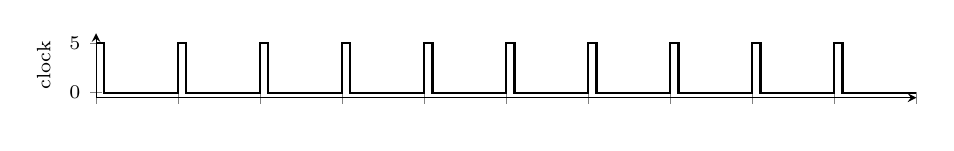
\begin{tikzpicture}
\begin{axis}[width=12cm,height=2.4cm,xmin=0,xmax=2,ymin=-0.5,ymax=6,
	axis lines=left,font=\scriptsize,ytick={0,5},ylabel={clock},
	xtick={0,0.2,...,2.0},xticklabels={}]
\addplot[black,thick,const plot] coordinates {(0,5) (0.02,0) (0.2,5) (0.22,0) (0.4,5) (0.42,0)
	(0.6,5) (0.62,0) (0.8,5) (0.82,0) (1.0,5) (1.02,0) (1.2,5) (1.22,0) (1.4,5) (1.42,0)
	(1.6,5) (1.62,0) (1.8,5) (1.82,0) (2.0,0)};
\end{axis}
\end{tikzpicture}
\end{center}
\bi
	\ite the output is a \textbf{staircase}: one step per sampling period
	\ite the value of each step is $\Vin$ at the \textbf{end} of the track phase
\ei
\nsl{The plot shows $\Vin = \SI{2}{\volt} + \SI{1.5}{\volt}\,\sin(2\pi\cdot
\SI{0.5}{\hertz}\cdot t)$ sampled at \SI{5}{\hertz}. The clock in the
timing row is high for one tenth of each period. The steps of $V_H$ start at
the falling clock edge, when the switch opens. (In the plot the short track
phases are not resolved.)}
\os{\newpage}

\item[{\rot\bf Terms}]~\\[-\lblskip]
\begin{center}
\begin{tikzpicture}[font=\sffamily\scriptsize,>=Stealth,x=1.1cm,y=1cm]
	% clock
	\draw[thick] (0,3) -- (1,3) -- (1,3.6) -- (4,3.6) -- (4,3) -- (9,3);
	\node[left] at (0,3.3) {clock};
	% Vh
	\draw[rwucyan,thick] (0,0.3) -- (1,0.3);
	\draw[rwuviolet,very thick] (1,0.3) .. controls (1.4,2.1) and (1.8,2.2) .. (2.6,2.25)
	   .. controls (3.2,2.3) and (3.6,2.3) .. (4,2.3);
	\draw[rwuviolet,very thick] (4,2.3) -- (4.1,2.05) -- (4.4,2.12) -- (9,1.9);
	\node[left] at (0,1.2) {$V_H$};
	\draw[dashed] (1,0) -- (1,3.8); \draw[dashed] (4,0) -- (4,3.8);
	\draw[dashed] (4.4,0) -- (4.4,2.2);
	\draw[<->] (1,-0.2) -- node[below]{acquisition time} (2.6,-0.2);
	\draw[<->] (4,-0.2) -- node[below]{\,aperture} (4.4,-0.2);
	\draw[<->] (6,2.4) -- node[above]{droop} (6,2.0);
	\node[align=center] at (2.5,3.9) {track};
	\node[align=center] at (6.5,3.9) {hold};
	\node[align=left,anchor=west] at (4.6,1.0) {pedestal (charge injection)\\and settling};
	\draw[->] (4.6,1.1) -- (4.15,2.0);
\end{tikzpicture}
\end{center}
\bi
	\ite \textbf{acquisition time}: track time needed until $V_H$ is within the error band (e.g.\ $\frac12\,\LSB$)
	\ite \textbf{aperture time}: delay between the hold command and the real opening of the switch; its variation is the \textbf{aperture jitter}
	\ite \textbf{pedestal}: step at the transition to hold; \textbf{droop}: slow change during hold
\ei
\os{\newpage}

\item[{\rot\bf Falstad: basic S\&H}]~\\[-\lblskip]
\bi
	\ite $\Vin = \SI{2}{\volt} + \SI{1.5}{\volt}\,\sin(2\pi\cdot\SI{0.5}{\hertz}\cdot t)$, $R_S = \SI{1}{\kilo\ohm}$, $C_H = \SI{1}{\micro\farad}$
	\ite clock rail: square wave \SI{5}{\hertz}, \SIrange{0}{5}{\volt}, duty cycle 0.1
	\ite held values: \SI{2.094}{\volt}, \SI{2.956}{\volt}, \SI{3.452}{\volt}, \SI{3.394}{\volt}, \SI{2.804}{\volt}
	\ite the scope shows $\Vin$, $V_H$ (label \texttt{Vhold}) and the clock
\ei
\falstad{sh_basic}
\nsl{The held values are the input voltages at the end of each track
window, $t = \SI{0.02}{\second}, \SI{0.22}{\second}, \ldots$ The simulation
shows them about \SI{5}{\milli\volt} lower, because the capacitor lags
behind a rising input by roughly the slope times the time constant
($\SI{4.7}{\volt\per\second}\cdot\SI{1}{\milli\second}$).}
\os{\newpage}
\end{description}

%%%%%%%%%%%%%%%%%%%%%%%%%%%%%%%%%%%%%%%%%%%%%%%%%%%%%%%%%%%%%%%%%%%%%%%%%%%
\section{Analog Switches}
%%%%%%%%%%%%%%%%%%%%%%%%%%%%%%%%%%%%%%%%%%%%%%%%%%%%%%%%%%%%%%%%%%%%%%%%%%%
\nsl{The switch of an S\&H stage is electronic. It must close and open on a
logic signal, have a low resistance when closed and an extremely high
resistance when open, and it must not disturb the stored charge. The
standard solution is a MOSFET, or two complementary MOSFETs in parallel
(transmission gate) \cite{sedra2020,horowitz2015}.\newpage}

\begin{description}
\item[{\rot\bf The MOSFET as a switch}]~\\[-\lblskip]
\begin{center}
\begin{circuitikz}[scale=0.85, transform shape]
  \node[nmos, rotate=-90] (m) at (2,0) {};
  \draw (0,0) node[left]{$\Vin$} to[short,o-] (m.S);
  \draw (m.D) -- (4,0) to[C, l=$C_H$] (4,-2) node[ground]{};
  \draw (4,0) to[short,-o] (5,0) node[right]{$V_H$};
  \draw (m.G) -- ++(0,0.5) node[above]{$V_G$: \SI{0}{\volt} / \SI{12}{\volt}};
\end{circuitikz}
\end{center}
\bi
	\ite n-channel MOSFET: conducts if $V_{GS} = V_G - \Vin > V_{th}$
	\ite on-resistance $R_\mathrm{on} \approx \frac{1}{k\,(V_{GS} - V_{th})}$: depends on $\Vin$!
	\ite near $\Vin \approx V_G - V_{th}$ the switch does not close any more
	\ite off: leakage currents in the pA \ldots nA range
\ei
\nsl{Source and drain of a MOSFET switch are interchangeable; the current
can flow in both directions. The gate voltage must be higher than the
largest input voltage plus the threshold voltage. If the input rises, the
gate-source voltage shrinks and the on-resistance grows. A single n-channel
switch is therefore good for signals near ground, a single p-channel
switch for signals near the positive supply.}
\os{\newpage}

\item[{\rot\bf CMOS transmission gate}]~\\[-\lblskip]
\begin{center}
\begin{circuitikz}[scale=0.85, transform shape]
  \draw (0,0) node[left]{$\Vin$} to[short,o-] (1.5,0) node[tgate, anchor=in](tg){};
  \draw (tg.out) to[short,-o] ++(1.5,0) node[right]{$V_H$};
  \draw (tg.gate) -- ++(0,0.4) node[above]{$\phi$};
  \draw (tg.notgate) -- ++(0,-0.4) node[below]{$\overline{\phi}$};
\end{circuitikz}
\begin{tikzpicture}
\begin{axis}[width=5.6cm,height=3.8cm,xmin=0,xmax=5,ymin=0,ymax=400,
	xlabel={$\Vin$ / V},ylabel={$R_\mathrm{on}$ / $\Omega$},axis lines=left,font=\scriptsize]
\addplot[rwucyan,thick,domain=0:3.3,samples=40] {100/(1-x/3.6)};
\addplot[rwuvioletlight,thick,domain=1.7:5,samples=40] {100/(1-(5-x)/3.6)};
\addplot[rwuviolet,very thick,domain=0:5,samples=60] {1/((x<3.5 ? (1-x/3.6)/100 : 0.0003) + (x>1.5 ? (1-(5-x)/3.6)/100 : 0.0003))};
\node[font=\tiny,rwucyandark] at (axis cs:0.9,330) {nMOS};
\node[font=\tiny,rwuviolet] at (axis cs:4.1,330) {pMOS};
\node[font=\tiny,rwuviolet] at (axis cs:2.5,120) {parallel};
\end{axis}
\end{tikzpicture}
\end{center}
\bi
	\ite nMOS and pMOS in parallel, driven with complementary signals
	\ite nMOS conducts well near \SI{0}{\volt}, pMOS near $V_{DD}$: together almost constant $R_\mathrm{on}$
	\ite integrated as CD4066, 74HC4066 (4 switches, $R_\mathrm{on}\approx$ \SIrange{50}{300}{\ohm}), DG4xx
\ei
\os{\newpage}

\item[{\rot\bf The analog switch in Falstad}]~\\[-\lblskip]
\bi
	\ite element \emph{Analog Switch} (models a FET switch / transmission gate)
	\bi
		\itee closed if the control input is above \SI{2.5}{\volt}
		\itee $R_\mathrm{on} = \SI{20}{\ohm}$, $R_\mathrm{off} = \SI{10}{\giga\ohm}$ (defaults, edit with a double click)
	\ei
	\ite no charge injection, no leakage: add them as extra elements if you want to see their effect
	\ite in our circuits: $R_S = \SI{1}{\kilo\ohm}$ in series
	\bi
		\itee limits the current from the op-amp output into the empty capacitor
		\itee isolates the op-amp from the large capacitive load (stability)
		\itee real lab switches have $R_\mathrm{on}$ of some \SI{100}{\ohm} anyway
	\ei
\ei
\nsl{The Falstad switch is ideal apart from its two resistances. A real
switch adds charge injection, leakage and a small coupling capacitance
across the open switch. We add these effects one at a time with discrete
elements (a capacitor from the clock to the hold node, a current source in
parallel to $C_H$) to see their influence separately.}
\os{\newpage}
\end{description}

%%%%%%%%%%%%%%%%%%%%%%%%%%%%%%%%%%%%%%%%%%%%%%%%%%%%%%%%%%%%%%%%%%%%%%%%%%%
\section{Designing the Hold Capacitor}
%%%%%%%%%%%%%%%%%%%%%%%%%%%%%%%%%%%%%%%%%%%%%%%%%%%%%%%%%%%%%%%%%%%%%%%%%%%
\nsl{The hold capacitor is the central design decision. Two requirements
pull in opposite directions. A small capacitor charges quickly in the track
phase, but it loses its voltage quickly through leakage currents in the
hold phase. A large capacitor holds its voltage well, but it may not be
charged completely in the short track window. Both requirements give a
limit for $C_H$; any value in between works, and we choose one with margin
on both sides.\newpage}

\begin{description}
\item[{\rot\bf Acquisition: charging in the track window}]~\\[-\lblskip]
\begin{center}
\begin{circuitikz}[scale=0.85, transform shape]
  \draw (0,0) node[ground]{} to[V, l=$\Vin$] (0,2)
        to[R, l=$R_S$] (2.2,2) to[R, l=$R_\mathrm{on}$] (4.4,2)
        to[C, l=$C_H$, v^=$V_H$] (4.4,0) -- (0,0);
\end{circuitikz}
\begin{tikzpicture}
\begin{axis}[width=6cm,height=3.6cm,xmin=0,xmax=6,ymin=0,ymax=4.4,
	xlabel={$t/\tau$},ylabel={$V_H$ / V},axis lines=left,font=\scriptsize,
	xtick={0,1,2,2.77,4,5,6},xticklabels={0,1,2,2.77,4,5,6}]
\addplot[rwuviolet,thick,domain=0:6,samples=60] {4*(1-exp(-x))};
\addplot[dashed,domain=0:6] {3.75};
\addplot[dashed] coordinates {(2.77,0) (2.77,3.75)};
\node[font=\tiny,anchor=west] at (axis cs:3.0,3.4) {$\SI{4}{\volt} - \frac12\,\LSB$};
\end{axis}
\end{tikzpicture}
\end{center}
\bi
	\ite $V_H(t) = \Vin\,(1-e^{-t/\tau})$ with $\tau = (R_S + R_\mathrm{on})\,C_H$
	\ite error after time $t$: $\Vin\,e^{-t/\tau}$; worst case: step over the full scale $V_\mathrm{FS}$
\ei
\os{\newpage}

\item[{\rot\bf Settling to $\frac12$ LSB}]~\\[-\lblskip]
\bi
	\ite requirement: $V_\mathrm{FS}\,e^{-t/\tau} \leq \frac12\,\LSB = \frac{V_\mathrm{FS}}{2^{N+1}}$
\ei
\keyeq{Acquisition time for $N$ bit}{$\displaystyle t_\mathrm{acq} = \tau\,\ln\left(2^{N+1}\right) = (N+1)\,\ln 2\cdot\tau \approx 0.69\,(N+1)\,\tau$}
\bi
	\ite $N = 3$: $t_\mathrm{acq} = 2.77\,\tau$; \quad $N = 8$: $6.2\,\tau$; \quad $N = 12$: $9.0\,\tau$; \quad $N = 16$: $11.8\,\tau$
	\ite design rule: $t_\mathrm{acq} \leq t_\mathrm{track}$ \quad$\Rightarrow$\quad
	$\displaystyle C_H \leq \frac{t_\mathrm{track}}{(R_S + R_\mathrm{on})\,\ln 2^{N+1}}$
	\ite example: $R_S + R_\mathrm{on} = \SI{1.02}{\kilo\ohm}$, $C_H = \SI{1}{\micro\farad}$: $\tau = \SI{1.02}{\milli\second}$, $t_\mathrm{acq} = \SI{2.83}{\milli\second}$ $\ll \SI{20}{\milli\second}$
\ei
\falstad{sh_acquisition}
\nsl{The Falstad example charges $C_H = \SI{1}{\micro\farad}$ from a
\SI{4}{\volt} source through \SI{1}{\kilo\ohm} plus the \SI{20}{\ohm} of
the switch. After one time constant ($t = \SI{1.02}{\milli\second}$) the
capacitor shows \SI{2.53}{\volt} (\SI{63}{\percent}), after
$t_\mathrm{acq} = \SI{2.83}{\milli\second}$ it reaches \SI{3.75}{\volt},
i.e.\ $\frac12\,\LSB$ below the final value, and at the end of the
\SI{20}{\milli\second} window it holds \SI{4.00}{\volt}. Use a time
constant of a few percent of the track window; the remaining time is
reserve for the settling of the op-amp and for tolerances.}
\os{\newpage}

\item[{\rot\bf Droop: losing charge in the hold phase}]~\\[-\lblskip]
\begin{center}
\begin{circuitikz}[scale=0.85, transform shape]
  \draw (0,2) node[left]{from switch (open)} to[short,o-] (1.5,2) -- (3,2)
        to[C, l_=$C_H$] (3,0) node[ground]{};
  \draw (3,2) -- (5,2) to[I, l=$I_\mathrm{leak}$] (5,0) -- (3,0);
  \draw (5,2) to[short,-o] (6.5,2) node[right]{$V_H$};
\end{circuitikz}
\end{center}
\bi
	\ite leakage currents: switch (off), capacitor dielectric, input bias current of the buffer, board surface
\ei
\keyeq{Droop}{$\displaystyle \frac{dV_H}{dt} = \frac{I_\mathrm{leak}}{C_H}
\qquad\Rightarrow\qquad \Delta V_\mathrm{droop} = \frac{I_\mathrm{leak}\,t_\mathrm{hold}}{C_H}
\qquad\Rightarrow\qquad C_H \geq \frac{I_\mathrm{leak}\,t_\mathrm{hold}}{\Delta V_\mathrm{max}}$}
\bi
	\ite $t_\mathrm{hold}$: until the conversion is finished; worst case the whole period $T_s - t_\mathrm{track}$
\ei
\os{\newpage}

\item[{\rot\bf Too small, right, too large}]~\\[-\lblskip]
\bi
	\ite Falstad: $\Vin = \SI{3}{\volt}$, $R_S = \SI{1}{\kilo\ohm}$, leakage $I_\mathrm{leak} = \SI{50}{\nano\ampere}$ (exaggerated)
\ei
\begin{center}
\small
\begin{tabular}{lccc}
\toprule
 & $C_H = \SI{10}{\nano\farad}$ & $C_H = \SI{1}{\micro\farad}$ & $C_H = \SI{100}{\micro\farad}$\\
\midrule
$\tau$ & \SI{10}{\micro\second} & \SI{1.02}{\milli\second} & \SI{102}{\milli\second}\\
charged in \SI{20}{\milli\second}? & yes & yes & only \SI{18}{\percent} per sample\\
droop in \SI{180}{\milli\second} & \SI{0.9}{\volt} & \SI{9}{\milli\volt} & \SI{0.09}{\milli\volt}\\
Falstad & \SI{3.00}{\volt} $\to$ \SI{2.10}{\volt} & \SI{3.00}{\volt} $\to$ \SI{2.99}{\volt} & \SI{0.534}{\volt}, \ldots, \SI{1.876}{\volt} (5th)\\
\bottomrule
\end{tabular}
\end{center}
\falstad{sh_capsize}
\nsl{The too large capacitor is a low-pass filter rather than a hold
stage: after every sample it has covered only \SI{18}{\percent} of the
remaining distance to the input voltage, $1-e^{-\SI{20}{\milli\second}/
\SI{102}{\milli\second}} = 0.178$. After five samples it shows
$\SI{3}{\volt}\,(1-0.822^5) = \SI{1.88}{\volt}$ instead of \SI{3}{\volt}.
The too small capacitor follows the input perfectly but loses
\SI{5}{\volt\per\second} in the hold phase. A real leakage current is much
smaller (pA to nA), so the lower limit for $C_H$ is usually far away; we
exaggerated it to make the effect visible.}
\os{\newpage}

\item[{\rot\bf Choosing $C_H$: the window}]~\\[-\lblskip]
\bi
	\ite upper limit from the acquisition, lower limit from the droop:
\ei
\keyeq{Hold capacitor}{$\displaystyle \frac{I_\mathrm{leak}\,t_\mathrm{hold}}{\Delta V_\mathrm{max}} \;\leq\; C_H \;\leq\; \frac{t_\mathrm{track}}{(R_S+R_\mathrm{on})\,\ln 2^{N+1}}$}
\bi
	\ite capstone values: $I_\mathrm{leak} = \SI{10}{\nano\ampere}$, $\Delta V_\mathrm{max} = \frac{1}{10}\,\LSB = \SI{50}{\milli\volt}$, $t_\mathrm{hold} = \SI{180}{\milli\second}$, $t_\mathrm{track} = \SI{20}{\milli\second}$, $R_S+R_\mathrm{on}=\SI{1.02}{\kilo\ohm}$
	\bi
		\itee $\SI{36}{\nano\farad} \leq C_H \leq \SI{7.1}{\micro\farad}$ \quad$\Rightarrow$\quad $C_H = \SI{1}{\micro\farad}$ (geometric middle, film capacitor)
	\ei
	\ite choose the capacitor type: polypropylene or polystyrene film (low leakage, low dielectric absorption), C0G ceramic for small values; no electrolytic capacitors
\ei
\nsl{Choosing a value in the geometric middle of the allowed window gives
the same safety factor (here about 7) against both limits. Electrolytic
capacitors are unsuitable: their leakage current is in the microampere
range, and their capacitance is poorly defined. Dielectric absorption is a
memory effect of the insulating material: after a fast change of voltage a
part of the charge comes back slowly from the dielectric, and the held
voltage creeps towards the previous value. Film capacitors with
polypropylene or polystyrene dielectric show very little of it.}
\os{\newpage}
\end{description}

\designcard{Sample and Hold}{%
\begin{itemize}\itemsep 0pt
\item structure: input follower $\to$ $R_S$ + switch $\to$ $C_H$ to ground $\to$ output follower
\item clock: $f_s$, short duty cycle; track $t_\mathrm{track} = D\,T_s$ (capstone: \SI{5}{\hertz}, \SI{10}{\percent}: \SI{20}{\milli\second})
\item charging: $\tau = (R_S+R_\mathrm{on})\,C_H$, settled to $\frac12\,\LSB$ after $\tau\ln 2^{N+1}$ ($N=3$: $2.77\,\tau$) $\leq t_\mathrm{track}$
\item droop: $\Delta V = I_\mathrm{leak}\,t_\mathrm{hold}/C_H \leq$ fraction of an LSB
\item pedestal: $\Delta V = C_{gd}\,\Delta V_\mathrm{clk}/(C_H + C_{gd})$; larger $C_H$ helps
\item capstone choice: $R_S = \SI{1}{\kilo\ohm}$, $C_H = \SI{1}{\micro\farad}$ film: $t_\mathrm{acq} = \SI{2.8}{\milli\second}$, droop \SI{1.8}{\milli\volt} at \SI{10}{\nano\ampere}
\end{itemize}}
\os{\newpage}

%%%%%%%%%%%%%%%%%%%%%%%%%%%%%%%%%%%%%%%%%%%%%%%%%%%%%%%%%%%%%%%%%%%%%%%%%%%
\section{Errors of a Real Sample and Hold}
%%%%%%%%%%%%%%%%%%%%%%%%%%%%%%%%%%%%%%%%%%%%%%%%%%%%%%%%%%%%%%%%%%%%%%%%%%%
\nsl{Besides incomplete charging and droop, a real S\&H stage shows a
number of smaller errors. They matter in fast and high-resolution
converters; in our slow 3-bit capstone they are negligible, but it is good
to know where they come from and which design parameter influences them
\cite{kester2005,jung2005}.\newpage}

\begin{description}
\item[{\rot\bf Charge injection (pedestal)}]~\\[-\lblskip]
\begin{center}
\begin{circuitikz}[scale=0.85, transform shape]
  \draw (0,2) node[left]{$\Vin$} to[short,o-] (0.5,2) to[R, l=$R_S$] (2.5,2)
        to[nos, name=sw] (4.5,2) -- (6,2) to[C, l=$C_H$] (6,0) node[ground]{};
  \draw (6,2) to[short,-o] (7,2) node[right]{$V_H$};
  \draw (sw.north) -- (sw.north |- 0,3.4) node[above]{clock \SI{5}{\volt} $\to$ \SI{0}{\volt}};
  \draw (sw.north |- 0,3.0) node[circ]{} -- (5.2,3.0) to[C, l=$C_{gd}$] (5.2,2) node[circ]{};
\end{circuitikz}
\end{center}
\bi
	\ite the gate of the switch is coupled to the hold node through $C_{gd}$ (and the channel charge)
	\ite when the switch opens, the clock step $\Delta V_\mathrm{clk}$ is divided by $C_{gd}$ and $C_H$:\\
	$\displaystyle \Delta V_\mathrm{ped} = -\Delta V_\mathrm{clk}\,\frac{C_{gd}}{C_{gd}+C_H} \approx -\frac{Q_\mathrm{inj}}{C_H}$
	\ite $C_{gd}=\SI{10}{\pico\farad}$, \SI{5}{\volt}: $C_H = \SI{1}{\nano\farad}$: \SI{-49.5}{\milli\volt}; $C_H = \SI{100}{\nano\farad}$: \SI{-0.5}{\milli\volt}
\ei
\falstad{sh_pedestal}
\nsl{The pedestal is a constant offset as long as the clock amplitude and
$C_{gd}$ are constant, so it can be calibrated. Its signal-dependent part
(the channel charge depends on $V_{GS}$) cannot. Remedies are a larger
$C_H$, small switches, a transmission gate (the charges of the n- and
p-channel transistor partly cancel), and dummy switches driven with the
inverted clock. In Falstad we model only the coupling capacitance; the
labels \texttt{Vhold\_1n} and \texttt{Vhold\_100n} show \SI{1.9505}{\volt}
and \SI{1.9995}{\volt} after the switch has opened, for an input of
\SI{2}{\volt}.}
\os{\newpage}

\item[{\rot\bf Feedthrough, aperture and jitter}]~\\[-\lblskip]
\bi
	\ite \textbf{feedthrough}: the open switch has a capacitance $C_\mathrm{ds}$; the input still reaches $C_H$:
	$\Delta V_H = \Delta\Vin\,\frac{C_\mathrm{ds}}{C_\mathrm{ds}+C_H}$
	\ite \textbf{aperture delay} $t_a$: the switch opens a little after the clock edge; constant, only shifts the sampling instant
	\ite \textbf{aperture jitter} $t_j$: random variation of the sampling instant
	\bi
		\itee error $\Delta V = \frac{dV}{dt}\,t_j$; sine: $\Delta V_\mathrm{max} = 2\pi f\hat V\,t_j$
		\itee requirement $\Delta V_\mathrm{max} < \frac12\,\LSB$: $\displaystyle t_j < \frac{1}{2\pi f\,2^{N+1}}\cdot\frac{V_\mathrm{FS}}{\hat V}$
		\itee example: 12 bit, full-scale sine of \SI{1}{\mega\hertz}: $t_j < \SI{19}{\pico\second}$
	\ei
	\ite \textbf{dielectric absorption}: held voltage creeps back towards the previous value
\ei
\nsl{For a full-scale sine $\hat V = V_\mathrm{FS}/2$ the jitter limit is
$t_j < 1/(2\pi f\,2^N)$. Jitter is the reason why fast converters need
clean, low-noise clock sources. For our \SI{5}{\hertz} system a jitter of
a millisecond is harmless (exercise~\ref{ex:sh-jitter}).}
\os{\newpage}
\end{description}

%%%%%%%%%%%%%%%%%%%%%%%%%%%%%%%%%%%%%%%%%%%%%%%%%%%%%%%%%%%%%%%%%%%%%%%%%%%
\section{The Buffered Sample and Hold}
%%%%%%%%%%%%%%%%%%%%%%%%%%%%%%%%%%%%%%%%%%%%%%%%%%%%%%%%%%%%%%%%%%%%%%%%%%%
\nsl{The bare switch and capacitor only work with an ideal source and an
ideal load. A real source has an internal resistance, for example the
output resistance of a passive anti-aliasing filter, and a real load draws
current, for example the input resistance of the converter or the
reference ladder of a flash converter. The cure is a voltage follower on
each side of the hold capacitor (chapter~5).\newpage}

\begin{description}
\item[{\rot\bf Follower -- switch -- capacitor -- follower}]~\\[-\lblskip]
\begin{center}
\begin{circuitikz}[scale=0.8, transform shape]
  \draw (0,0) node[op amp, noinv input up](a1){};
  \draw (a1.+) -- ++(-0.6,0) node[left]{$\Vin$};
  \draw (a1.-) -- ++(0,0.9) -| (a1.out);
  \draw (a1.out) to[R, l=$R_S$] ++(2,0) to[nos, l=$S$, name=sw] ++(1.8,0) coordinate(h)
        to[short,*-] ++(1.2,0) coordinate(b2in);
  \draw (h) to[C, l_=$C_H$] ++(0,-1.8) node[ground]{};
  \draw (b2in) ++(1.2,-0.5) node[op amp, noinv input up](a2){};
  \draw (b2in) |- (a2.+);
  \draw (a2.-) -- ++(0,-0.8) -| (a2.out);
  \draw (a2.out) to[short,-o] ++(0.6,0) node[right]{$\Vout$};
  \draw (sw.north) ++(0,0.2) -- ++(0,0.6) node[above]{clock};
\end{circuitikz}
\end{center}
\bi
	\ite \textbf{input buffer}: the charging current comes from the op-amp, not from the signal source
	\ite \textbf{output buffer}: draws (almost) no current from $C_H$; only its input bias current adds to the leakage
\ei
\os{\newpage}

\item[{\rot\bf Why both buffers are needed}]~\\[-\lblskip]
\bi
	\ite without buffers: source $R_i = \SI{10}{\kilo\ohm}$, load $R_L = \SI{100}{\kilo\ohm}$ (e.g.\ ADC input), $\Vin = \SI{3}{\volt}$
	\bi
		\itee track: $\tau = (R_i\parallelto R_L)\,C_H = \SI{9.1}{\milli\second}$, final value $\SI{3}{\volt}\cdot\frac{100}{110}=\SI{2.73}{\volt}$
		\itee after \SI{20}{\milli\second}: \SI{2.425}{\volt}
		\itee hold: discharge through $R_L$, $\tau = \SI{100}{\milli\second}$: \SI{0.401}{\volt} after \SI{180}{\milli\second}
	\ei
	\ite with buffers: \SI{3.000}{\volt} during the whole period
\ei
\falstad{sh_buffered}
\nsl{The unbuffered circuit fails in three ways at once: the source and the
load form a voltage divider, the source resistance makes the charging slow,
and the load discharges the capacitor in the hold phase. With buffers the
source only sees the high input resistance of the first follower, and the
capacitor only sees the high input resistance of the second follower.
For the output buffer choose an op-amp with FET input (bias current in the
pA range); its bias current is part of $I_\mathrm{leak}$.}
\os{\newpage}

\item[{\rot\bf The sampling clock}]~\\[-\lblskip]
\begin{center}
\begin{tikzpicture}[font=\sffamily\scriptsize,>=Stealth,x=0.5cm,y=0.5cm]
	\node[left] at (0,0.5) {clock};
	\draw[thick] (0,0) \foreach \k in {0,10,20} { -- (\k,0) -- (\k,1) -- (\k+1,1) -- (\k+1,0) } -- (30,0);
	\node[left] at (0,-1.2) {switch};
	\foreach \k in {0,10,20} {
		\draw[fill=rwucyan!30] (\k,-1.7) rectangle (\k+1,-0.7);
		\draw (\k+1,-1.7) rectangle (\k+10,-0.7) node[midway]{hold: $V_H$ constant, ADC reads};
	}
	\draw[<->] (0,1.5) -- (1,1.5) node[right]{$t_\mathrm{track}=\SI{20}{\milli\second}$};
	\draw[<->] (0,2.6) -- node[above]{$T_s=\SI{200}{\milli\second}$} (10,2.6);
	\draw[dashed] (10,2.6) -- (10,1);
\end{tikzpicture}
\end{center}
\bi
	\ite square wave with a short duty cycle $D = t_\mathrm{track}/T_s$
	\ite Falstad: rail with waveform \emph{square}, \SI{5}{\hertz}, amplitude \SI{2.5}{\volt}, offset \SI{2.5}{\volt}, duty cycle 0.1
	\ite in hardware: 555 timer or microcontroller output; 0/5 V logic level drives the switch
	\ite the ADC result is read in the hold phase (e.g.\ in the middle or at the end)
\ei
\nsl{A short track phase keeps the output constant for most of the period.
The track phase must not be too short either: it must be longer than the
acquisition time. With $D = 0.1$ at \SI{5}{\hertz} we have
\SI{20}{\milli\second} for charging and \SI{180}{\milli\second} of stable
output.}
\os{\newpage}

\item[{\rot\bf Sampling a ramp}]~\\[-\lblskip]
\begin{center}
\begin{tikzpicture}
\begin{axis}[width=10cm,height=4.2cm,xmin=0,xmax=1.2,ymin=0,ymax=4.4,
	xlabel={$t$ / s},ylabel={$V$ / V},axis lines=left,font=\scriptsize,
	xtick={0,0.2,...,1.2},xticklabel style={/pgf/number format/fixed},
	legend style={at={(0.02,0.98)},anchor=north west,draw=none,fill=none}]
\addplot[rwucyan,thick] coordinates {(0,0) (1,4) (1.2,3.2)};
\addlegendentry{$\Vin$ (triangle, \SI{4}{\volt\per\second})}
\addplot[rwuviolet,very thick,const plot] coordinates {(0,0) (0.02,0.08) (0.22,0.88) (0.42,1.68) (0.62,2.48) (0.82,3.28) (1.02,3.92) (1.2,3.92)};
\addlegendentry{$\Vout$}
\end{axis}
\end{tikzpicture}
\end{center}
\bi
	\ite buffered S\&H, triangle \SIrange{0}{4}{\volt} at \SI{0.5}{\hertz}: steps of $\SI{4}{\volt\per\second}\cdot\SI{0.2}{\second} = \SI{0.8}{\volt}$
	\ite Falstad: \SI{0.08}{\volt}, \SI{0.88}{\volt}, \SI{1.68}{\volt}, \SI{2.48}{\volt}, \SI{3.28}{\volt}
\ei
\falstad{sh_staircase}
\nsl{A step of \SI{0.8}{\volt} is larger than one LSB of the 3-bit
converter (\SI{0.5}{\volt}): consecutive samples skip codes. This is no
error of the S\&H stage. The input simply changes too fast for the
sampling rate; such fast signals have to be removed by the anti-aliasing
filter (see the sampling theorem in the next chapter).}
\os{\newpage}

\item[{\rot\bf Practical hints}]~\\[-\lblskip]
\bi
	\ite op-amps: rail-to-rail output for the full range \SIrange{0}{4}{\volt} on a single \SI{5}{\volt} supply, FET input for the output buffer
	\ite guard ring around the hold node on the PCB: surface leakage
	\ite integrated S\&H amplifiers (LF398, AD783) contain both buffers and the switch; only $C_H$ is external
	\ite in most modern ADCs (SAR, sigma-delta) the S\&H is built in: a switched capacitor array at the input
	\bi
		\itee the driving op-amp must recharge this capacitor in the acquisition time: the same calculation as above
	\ei
\ei
\nsl{The LF398 is a classic monolithic S\&H amplifier; its data sheet
contains curves for acquisition time and droop rate as functions of $C_H$
that are a good illustration of this chapter. Modern SAR converters in
microcontrollers sample with an internal capacitor of a few picofarads;
the source resistance must be low enough that this capacitor charges to
$\frac12\,\LSB$ within the programmed sampling time, which is exactly the
calculation $t_\mathrm{acq} = \tau\ln 2^{N+1}$.}
\os{\newpage}
\end{description}

%%%%%%%%%%%%%%%%%%%%%%%%%%%%%%%%%%%%%%%%%%%%%%%%%%%%%%%%%%%%%%%%%%%%%%%%%%%
\section{Exercises}
%%%%%%%%%%%%%%%%%%%%%%%%%%%%%%%%%%%%%%%%%%%%%%%%%%%%%%%%%%%%%%%%%%%%%%%%%%%

\exercise{Choosing the hold capacitor for $f_s = \SI{5}{\hertz}$}\label{ex:sh-cap}
A buffered S\&H stage samples at $f_s = \SI{5}{\hertz}$ with a clock duty
cycle of \SI{10}{\percent}. The charging path consists of
$R_S = \SI{1}{\kilo\ohm}$ and a switch with $R_\mathrm{on} = \SI{20}{\ohm}$.
The total leakage current at the hold node (switch, capacitor, buffer bias)
is at most $I_\mathrm{leak} = \SI{10}{\nano\ampere}$. The stage drives a
3-bit converter with $V_\mathrm{FS} = \SI{4}{\volt}$.
\begin{talist}
\ta Calculate the track and hold times.
\ta The capacitor must settle to $\frac12\,\LSB$ for a full-scale step
	within the track phase. Find the upper limit for $C_H$.
\ta The droop during the hold phase must stay below $\frac{1}{10}\,\LSB$.
	Find the lower limit for $C_H$.
\ta Choose $C_H$ and calculate acquisition time and droop for your choice.
\ta Check the charging curve in Falstad.
\end{talist}

\begin{solution}
\begin{talist}
\ta $T_s = 1/f_s = \SI{200}{\milli\second}$, $t_\mathrm{track} = 0.1\cdot T_s = \SI{20}{\milli\second}$,
	$t_\mathrm{hold} = \SI{180}{\milli\second}$.
\ta $\LSB = \SI{4}{\volt}/8 = \SI{0.5}{\volt}$. Settling to $\frac12\,\LSB$ needs
	$t = \tau\ln 2^{4} = 2.77\,\tau \leq \SI{20}{\milli\second}$, so
	$\tau \leq \SI{7.21}{\milli\second}$ and
	$C_H \leq \SI{7.21}{\milli\second}/\SI{1020}{\ohm} = \SI{7.1}{\micro\farad}$.
\ta $\Delta V_\mathrm{max} = \SI{50}{\milli\volt}$:
	$C_H \geq I_\mathrm{leak}\,t_\mathrm{hold}/\Delta V_\mathrm{max}
	= \SI{10}{\nano\ampere}\cdot\SI{0.18}{\second}/\SI{50}{\milli\volt} = \SI{36}{\nano\farad}$.
\ta The window is \SI{36}{\nano\farad} \ldots \SI{7.1}{\micro\farad}; the geometric middle
	is about \SI{0.5}{\micro\farad}. We choose $C_H = \SI{1}{\micro\farad}$ (film capacitor).
	Then $\tau = \SI{1.02}{\milli\second}$, $t_\mathrm{acq} = 2.77\,\tau = \SI{2.83}{\milli\second}$
	(seven times faster than required) and
	$\Delta V_\mathrm{droop} = \SI{10}{\nano\ampere}\cdot\SI{0.18}{\second}/\SI{1}{\micro\farad}
	= \SI{1.8}{\milli\volt}$ (28 times smaller than allowed).
\ta \falstad{sh_acquisition}\newline With a \SI{4}{\volt} input, \texttt{Vhold} shows
	\SI{2.53}{\volt} after \SI{1.02}{\milli\second}, \SI{3.75}{\volt} after
	\SI{2.83}{\milli\second} and \SI{4.00}{\volt} at the end of the track phase.
	(Pause the simulation and use the scope, or reduce the simulation speed.)
\end{talist}
\end{solution}

\exercise{Droop and a too large capacitor}
The S\&H stage of exercise~\ref{ex:sh-cap} has an (exaggerated) leakage current of
\SI{50}{\nano\ampere}. The input is a constant \SI{3}{\volt}.
\begin{talist}
\ta Calculate the droop rate and the voltage at the end of the first hold
	phase for $C_H = \SI{10}{\nano\farad}$ and for $C_H = \SI{1}{\micro\farad}$.
\ta With $C_H = \SI{100}{\micro\farad}$, which fraction of the remaining
	difference is charged in one track window? Calculate the held voltage after
	the first and after the fifth sample (leakage negligible).
\ta Compare with Falstad.
\end{talist}

\begin{solution}
\begin{talist}
\ta $C_H = \SI{10}{\nano\farad}$: $dV/dt = \SI{50}{\nano\ampere}/\SI{10}{\nano\farad} = \SI{5}{\volt\per\second}$,
	droop in \SI{180}{\milli\second}: \SI{0.9}{\volt}, the held voltage falls from \SI{3.00}{\volt} to \SI{2.10}{\volt}.
	$C_H = \SI{1}{\micro\farad}$: \SI{50}{\milli\volt\per\second}, droop \SI{9}{\milli\volt}.
\ta $\tau = \SI{1.02}{\kilo\ohm}\cdot\SI{100}{\micro\farad} = \SI{102}{\milli\second}$,
	fraction $a = 1-e^{-20/102} = 0.178$. After $n$ samples
	$V_n = \SI{3}{\volt}\,(1-(1-a)^n)$: $V_1 = \SI{0.534}{\volt}$,
	$V_5 = \SI{3}{\volt}\,(1-0.822^5) = \SI{1.876}{\volt}$.
\ta \falstad{sh_capsize}\newline \texttt{V\_10n} drops from \SI{3.00}{\volt} to \SI{2.10}{\volt} in every hold phase,
	\texttt{V\_1u} loses \SI{9}{\milli\volt} (\SI{3.00}{\volt} $\to$ \SI{2.99}{\volt}),
	\texttt{V\_100u} climbs in steps: \SI{0.534}{\volt} after the first, \SI{1.876}{\volt} after the fifth sample.
\end{talist}
\end{solution}

\exercise{Unbuffered sample and hold}
A switch and $C_H = \SI{1}{\micro\farad}$ are connected directly between a
source ($\Vin = \SI{3}{\volt}$, internal resistance $R_i = \SI{10}{\kilo\ohm}$)
and a load $R_L = \SI{100}{\kilo\ohm}$. Clock: \SI{5}{\hertz}, \SI{10}{\percent}.
Neglect $R_\mathrm{on}$.
\begin{talist}
\ta Draw the equivalent circuit for the track phase and calculate its final
	value and time constant.
\ta Calculate $V_H$ at the end of the first track phase and at the end of
	the first hold phase.
\ta How does the buffered circuit change the result? Check in Falstad.
\end{talist}

\begin{solution}
\begin{talist}
\ta Thevenin equivalent seen by $C_H$: $V_\mathrm{th} = \SI{3}{\volt}\cdot\frac{100}{110} = \SI{2.727}{\volt}$,
	$R_\mathrm{th} = R_i\parallelto R_L = \SI{9.09}{\kilo\ohm}$, $\tau = \SI{9.09}{\milli\second}$.
\ta End of track: $V_H = \SI{2.727}{\volt}\,(1-e^{-20/9.09}) = \SI{2.425}{\volt}$.
	Hold: $C_H$ discharges through $R_L$ with $\tau = \SI{100}{\milli\second}$:
	$V_H = \SI{2.425}{\volt}\cdot e^{-1.8} = \SI{0.401}{\volt}$.
\ta The input follower removes the divider and the slow charging, the output follower
	removes the discharge: $V_\mathrm{out} = \SI{3.000}{\volt}$ throughout.
	\newline\falstad{sh_buffered}\newline \texttt{Vout\_unbuf} shows \SI{2.425}{\volt} and
	\SI{0.401}{\volt}, \texttt{Vout\_buf} \SI{3.000}{\volt}.
\end{talist}
\end{solution}

\exercise{Pedestal error}
The gate of the switch has a coupling capacitance $C_{gd} = \SI{10}{\pico\farad}$
to the hold node. The clock falls from \SI{5}{\volt} to \SI{0}{\volt} when the switch opens.
\begin{talist}
\ta Calculate the pedestal for $C_H = \SI{1}{\nano\farad}$ and $C_H = \SI{100}{\nano\farad}$.
\ta Which $C_H$ is needed for a pedestal below $\frac12\,\LSB$ of a 12-bit
	converter with $V_\mathrm{FS} = \SI{4}{\volt}$?
\ta Is the pedestal a problem for the 3-bit capstone with $C_H = \SI{1}{\micro\farad}$?
\end{talist}

\begin{solution}
\begin{talist}
\ta $\Delta V = -\SI{5}{\volt}\cdot\frac{\SI{10}{\pico\farad}}{\SI{1.01}{\nano\farad}} = \SI{-49.5}{\milli\volt}$;
	with \SI{100}{\nano\farad}: \SI{-0.50}{\milli\volt}.
	\newline\falstad{sh_pedestal}: \SI{2}{\volt} input, held values \SI{1.9505}{\volt} and \SI{1.9995}{\volt}.
\ta $\frac12\,\LSB = \SI{4}{\volt}/2^{13} = \SI{0.49}{\milli\volt}$:
	$C_H \geq \SI{5}{\volt}\cdot\SI{10}{\pico\farad}/\SI{0.49}{\milli\volt} = \SI{0.1}{\micro\farad}$.
\ta $\Delta V = \SI{50}{\micro\volt}$, i.e.\ $10^{-4}$ of an LSB of \SI{0.5}{\volt}: no problem.
\end{talist}
\end{solution}

\exercise{Ramp input and step size}
A buffered S\&H stage ($f_s = \SI{5}{\hertz}$) samples a triangle that rises from
\SI{0}{\volt} to \SI{4}{\volt} in \SI{1}{\second}.
\begin{talist}
\ta Calculate the height of the steps of the output staircase.
\ta The sampling instants are at the end of the track windows,
	$t_k = \SI{20}{\milli\second} + k\cdot\SI{200}{\milli\second}$. List the first five held values.
\ta What is the maximum slope of the input if consecutive samples may differ by
	at most one LSB of the 3-bit converter? What does this mean for a sine with an
	amplitude of \SI{2}{\volt}?
\end{talist}

\begin{solution}
\begin{talist}
\ta $\SI{4}{\volt\per\second}\cdot\SI{0.2}{\second} = \SI{0.8}{\volt}$.
\ta $V(t_k) = \SI{4}{\volt\per\second}\cdot t_k$: \SI{0.08}{\volt}, \SI{0.88}{\volt}, \SI{1.68}{\volt},
	\SI{2.48}{\volt}, \SI{3.28}{\volt}.
	\newline\falstad{sh_staircase}: \texttt{Vout} shows the same values (\SI{4}{\milli\volt} lower,
	because $C_H$ lags by $\tau\cdot\SI{4}{\volt\per\second}$).
\ta $\SI{0.5}{\volt}/\SI{0.2}{\second} = \SI{2.5}{\volt\per\second}$.
	Sine: $2\pi f\cdot\SI{2}{\volt} \leq \SI{2.5}{\volt\per\second}$ gives
	$f \leq \SI{0.2}{\hertz}$. Faster signals are still sampled correctly as long as
	$f < f_s/2$ (next chapter), but the codes of neighbouring samples jump.
\end{talist}
\end{solution}

\exercise{Aperture jitter}\label{ex:sh-jitter}
The \SI{5}{\hertz} clock of the capstone comes from a microcontroller whose
software has a timing uncertainty of $t_j = \SI{1}{\milli\second}$. The input
is a sine with $\hat V = \SI{2}{\volt}$ and $f = \SI{2.5}{\hertz}$
(the highest frequency the anti-aliasing filter passes).
\begin{talist}
\ta Calculate the maximum sampling error caused by the jitter.
\ta Compare with $\frac12\,\LSB$ of the 3-bit converter.
\ta Which jitter would a 16-bit converter tolerate for the same signal
	($V_\mathrm{FS} = \SI{4}{\volt}$)?
\end{talist}

\begin{solution}
\begin{talist}
\ta $\Delta V_\mathrm{max} = 2\pi f\hat V\,t_j = 2\pi\cdot\SI{2.5}{\hertz}\cdot\SI{2}{\volt}\cdot\SI{1}{\milli\second}
	= \SI{31}{\milli\volt}$.
\ta $\frac12\,\LSB = \SI{250}{\milli\volt}$: the jitter error is eight times smaller, harmless.
\ta $\frac12\,\LSB = \SI{4}{\volt}/2^{17} = \SI{30.5}{\micro\volt}$:
	$t_j < \SI{30.5}{\micro\volt}/(2\pi\cdot\SI{2.5}{\hertz}\cdot\SI{2}{\volt}) = \SI{0.97}{\micro\second}$.
	A software-timed clock is no longer good enough; a hardware timer is needed.
\end{talist}
\end{solution}

%%% Local Variables:
%%% mode: latex
%%% TeX-master: "docu"
%%% End:
